% !TEX encoding = UTF-8 Unicode
\documentclass[a4paper]{article}
%\usepackage[T1]{fontenc}     % För svenska bokstäver
\usepackage[utf8]{inputenc}  % Teckenkodning UTF8
%\usepackage[swedish]{babel}  % För svensk avstavning och svenska
                             % rubriker (t ex Innehållsförteckning)
\usepackage{fancyvrb}        % För programlistor med tabulatorer
\fvset{tabsize=4}            % Tabulatorpositioner
\fvset{fontsize=\small}      % Lagom storlek för programlistor
\usepackage[labelfont=bf]{caption}
\usepackage{hyperref}
\usepackage{graphicx}         % För att inkludera bilder.
\usepackage{float}

\title{Lego Mindstorm Project: Lego Segway\\
Course FRTN01 - Real time systems}
\author{Simon Wallström, dat11swa@student.lu.se\\
Adam Dalentoft, dat11ada@student.lu.se\\
Jonathan Karlsson, ada09jka@student.lu.se}
%\date{1 augusti 1994}        % Blir dagens datum om det utelämnas
\begin{document}              % Början på dokumentet

\maketitle
\thispagestyle{empty}
\newpage
\setcounter{page}{1}
\tableofcontents
\newpage
\section{Introduction}
The goal of this project is to build and control a two-wheeled robot - a Lego Segway - using NXT Lego Mindstorm 2.0. A segway is an unstable system that constantly needs to be regulated to work. To regulate this system several parameters is required. It is important to know the mass and specifications of the hardware that is used and the physics and movements in the system. Basically how it works is that the the robot tilts and the angle is measured. Thereafter the angle is processed by the controller to calculate the required change in degree for the wheels. It is possible to control the segway in a few different ways. One way is to use pole placing and feedback control. Even though this is a good way to regulate the system it is hard to realize. Therefore the structure that will be described in this report uses two PID controllers, one for the wheel position and one for the angle of the robot.\\

\begin{figure}[H]
  \centering
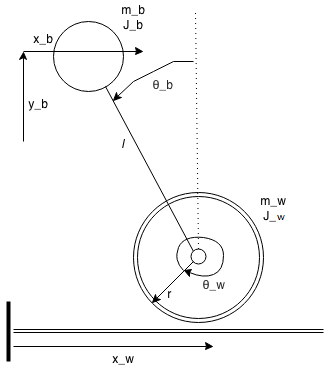
\includegraphics[scale=0.8]{pic/segway.png}
\caption{el caprioneE}
\end{figure}

Before the implementation can begin it is a good idea to set up a model of the process. The process is described in the picture, including the different variables that is needed to calculate the movements in the system. These variables are the used to calculate the state-space form for the system, describing the equation L = T - V. The state-space form of the system can thereafter be used in matlab and simulink to describe a control system for the segway. Simulink can also be used to make a simulation of the calculated system to determine parameters for the PID-controllers. \\

To implement the controller a Java version for Lego NXT is used called LeJOS. There are several alternatives in other languages but this is the only widely known Java VM. LeJOS provides classes for the most common hardware to the Lego NXT.  \\

To measure the angles a gyroscope and an accelerometer are used. The gyroscope measure the angle velocity and the integrated value gives the angle of the tilted segway. However the gyroscopes raw value drifts and therefore the accelerometer is required to compensate for this. Rest of the hardware is standard nxt motors and base unit.



\section{Program structure}
The program uses threads to realize a real time controlled system. 


\section{Control design}
As mentioned in the introduction the controller will contain two PID-controllers. They are connected in a cascade to regulate the two angles, tilt angle and wheel angle. The inner loop controls the tilt angle and the outer controls the wheel movement. 

\section{User information}
The segway does not have a user interface except the small screen and the buttons on the front of the base unit. When the segway is in motion these become a rather impractical way of controlling the system. Therefore the system is started before it is put down. It is however possible to change mode with the buttons from stand still mode and a mode that changes the reference value to make the robot move forward and backward. The monitor give small messages to inform the user how to handle the robot and what is happening in the system.

The program should be pre-installed on the machine.

\section{Results}
Inget funkar.


\section{Conclution}
Fuck everything, LEGO isn’t funny anymore :(


\end{document}                  % Slut på dokumentet



%\begin{figure}[H]
%  \centering
%\includegraphics[scale=0.8]{xXx.png}
%\caption{el caprioneE}
%\end{figure}